%%% MORITZ 2.5' %%%

\section{Doppelresonanz}
\subsection{Grundlagen: Optisches Pumpen}


\begin{frame}
\frametitle{Optisches Pumpen}
\setbeamerfont{myfont}{size*=45}
\usebeamerfont{myfont}

  \begin{figure}
    \centering
    \def\svgwidth{0.45\textwidth}
    \input{../img/termschema.pdf_tex}
    \caption{Termschema.}
\end{figure}
\end{frame}




\begin{frame}
\frametitle{Optisches Pumpen}

\begin{figure}[H]
\begin{center}
  \includegraphics[width=\textwidth]{../img/optPumpen.png}
  \caption{ca.}
\end{center}
\end{figure}
%TODO neues Bild mit Inkscape?

\end{frame}

\subsection{Aufbau}
\begin{frame}
\frametitle{Aufbau: Doppelresonanz}

\setbeamerfont{myfont}{size*=80}
\usebeamerfont{myfont}
\begin{figure}
    \centering
    \def\svgwidth{\textwidth}
    \input{../img/aufbauDR.pdf_tex}
    \caption{Aufbau zur Messung der Doppelresonanz.}
\end{figure}
\usebeamerfont{standard}

\begin{itemize}
  \item \textbf{\textlambda/4-Plättchen:} Erzeugung von zirkular polarisiertem Licht
  \item \textbf{Spule 1:} Einstellbarer Gleichstrom
  \item \textbf{Spule 2:} Sinusförmiger Strom
  \item \textbf{Spule 4:} Kompensation von vertikalem Erdmagnetfeld
  \item \textbf{RF-Sender:} Einstrahlung von elmag. Wechselfeld in die Messzelle
\end{itemize}

\end{frame}



%%% BEN 2.5' %%%

\subsection{Messung}

\begin{frame}
\frametitle{Messung: Doppelresonanz}
\begin{figure}
\begin{center}
  \includegraphics[width=\textwidth]{../img/06.pdf}
  \caption{Starke Modulation des Magnetfelds in Strahlrichtung mit Spule~2 (blau).
   Im Photodiodensignal (schwarz) sind vier Doppelresonanz-Peaks sowie
   zwei Dehmelt-Peaks pro Modulationsperiode sichtbar.}
  \label{img:dehmeltrf}
\end{center}
\end{figure}
\end{frame}

\begin{frame}
\frametitle{Messung: Doppelresonanz}
\begin{figure}
\begin{center}
    \includegraphics[width=\textwidth]{../img/07.pdf}
    \caption{Gleiches Setup wie bei \autoref{img:dehmeltrf}, aber ohne RF-Signal.
    Die leicht asymmetrischen Dehmelt-Peaks sind weiterhin vorhanden.}
    \label{img:dehmelt}
\end{center}
\end{figure}
\end{frame}

\begin{frame}
\frametitle{Messung: Doppelresonanz}
\begin{figure}
\begin{center}
  \includegraphics[width=\textwidth]{../img/11.pdf}
  \caption{Doppelresonanz-Absorptionssignal bei kleiner Magnetfeldmodulation:
  Falsche Einstellung des Gleichstroms in Spule~1,
  die Absorptionen sind nicht äquidistant.}
  \label{img:rfwrong}
\end{center}
\end{figure}
\end{frame}

\begin{frame}
\frametitle{Messung: Doppelresonanz}
\begin{figure}
\begin{center}
  \includegraphics[width=\textwidth]{../img/08.pdf}
  \caption{Doppelresonanz-Absorptionssignal bei kleiner Magnetfeldmodulation:
  Korrekte Einstellung des Gleichstroms in Spule~1,
  die Absorptionen sind daher äquidistant.}
  \label{img:rfcorrect}
\end{center}
\end{figure}
\end{frame}

\subsection{Auswertung}
\begin{frame}
\frametitle{Auswertung: Doppelresonanz}
  
\end{frame}